Recurrent Neural Network (RNN) is distinct by its memory, taking input sequence with no predetermined size. Its past predictions influence currently generated output. Thus for the same input, RNN could produce different results depending on previous inputs in the sequence \cite{rnnDSmedium}.

RNNs features make it commonly used in fields such as speech recognition, image captioning, natural language processing, or language translation. Some of the popular being, for example, Siri, Google Translate or Google Voice search \cite{ibmrnn}.

As previously mentioned, RNN takes into consideration information from previous inputs. Let us look at the idiom "feeling under the weather", where for it to make sense, words have to be in a specific order. RNN needs to account for each word's positions and use its information to predict the next word in the sequence. Each timestep represents a single word. In our case, the third timestep represents "the". Its hidden state holds information of previous inputs, "feeling" and "under" \cite{ibmrnn}.

\begin{figure}[h]
	\centering
    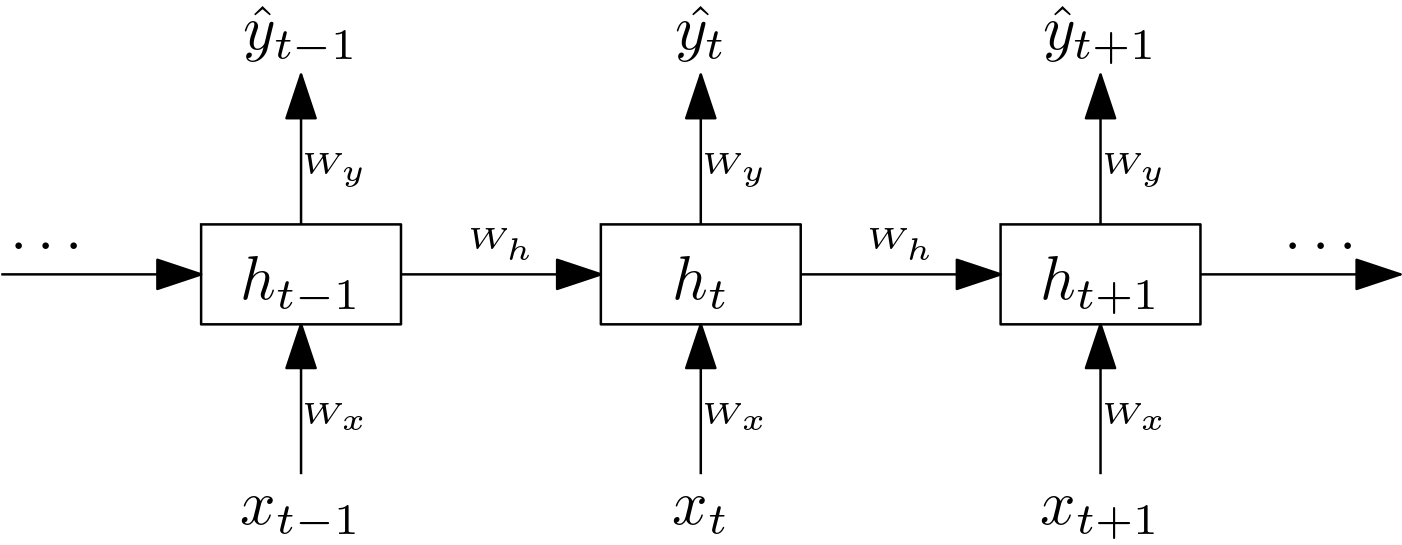
\includegraphics[width=12cm]{rnn_u.png}
	\caption{Unrolled structure of RNN \cite{matous}}
	\label{fig:rnn}
\end{figure}


Figure 1.4 shows the network for each timestep, i.e., at time $t$, the input $\vec{x_t}$ goes into the network to produce output $\hat{y}_t$, the next timestep of the input is $x_{t+1}$ with additional input from the previous time step from the hidden state $h_{t}$. This way, the neural network looks at the current input and has the context from the previous inputs.
With this structure, recurrent units hold the past values, referred to as memory. Making it possible to work with a context in the data \cite{rnnin6}.

The recurrent unit is calculated as follows:

\begin{equation}
    {h_t = f(W_{x}x_t + W_{h}h_{t-1}+\vec{b_h})}
\end{equation}

$f()$ being the activation function, $W_x,W_h$ are weight matrixes, $x_t$ is the input, and $\vec{b_h}$ is the vector of bias parameters. Unit at time step $t=0$ is initialized to $(0,0,...,0)$. The output $\hat{y_t}$ is then calculated as:

\begin{equation}
    {\hat{y}_t = g(W_{y}h_t + \vec{b_y})}
\end{equation}

$g()$ also being an activation function, usually being softmax to ensure the output is in the desired class range. $W_y$ is the weight matrix and $\vec{b_y}$ being a vector of biases determined during the learning process.

Training RNNs uses a modified version of the backpropagation algorithm called \textit{backpropagation through time} (BPTT), working by unrolling the RNN \cite{Goodfellow-et-al-2016}, calculating the losses across time steps, then updating the weights with the backpropagation algorithm. More on RNN in \cite{lipton2015critical} by Lipton et al.


\subsubsection{Bidirection Recurrent Neural Networks}


Bidirectional Recurrent Neural Networks (BRNN) allow training the network using all available input information in the past and future of a specific time frame. Oppose to regular RNN, where its hidden state is determined only by the prior states. The idea behind BRNN is splitting the hidden state into two. One is responsible for the positive time direction, \textit{forward states}, and the other for the negative time direction, \textit{backward states}.

BRNN’s training generally starts with processing forward, and backward states before output neurons are passed, \textit{forward pass}. Following with \textit{backward pass}, where output neurons are processed first, and forward and backward states after. Weights are then updated after completing forward pass and backward pass \cite{schusterbdrnn}.

\begin{figure}[h]
	\centering
    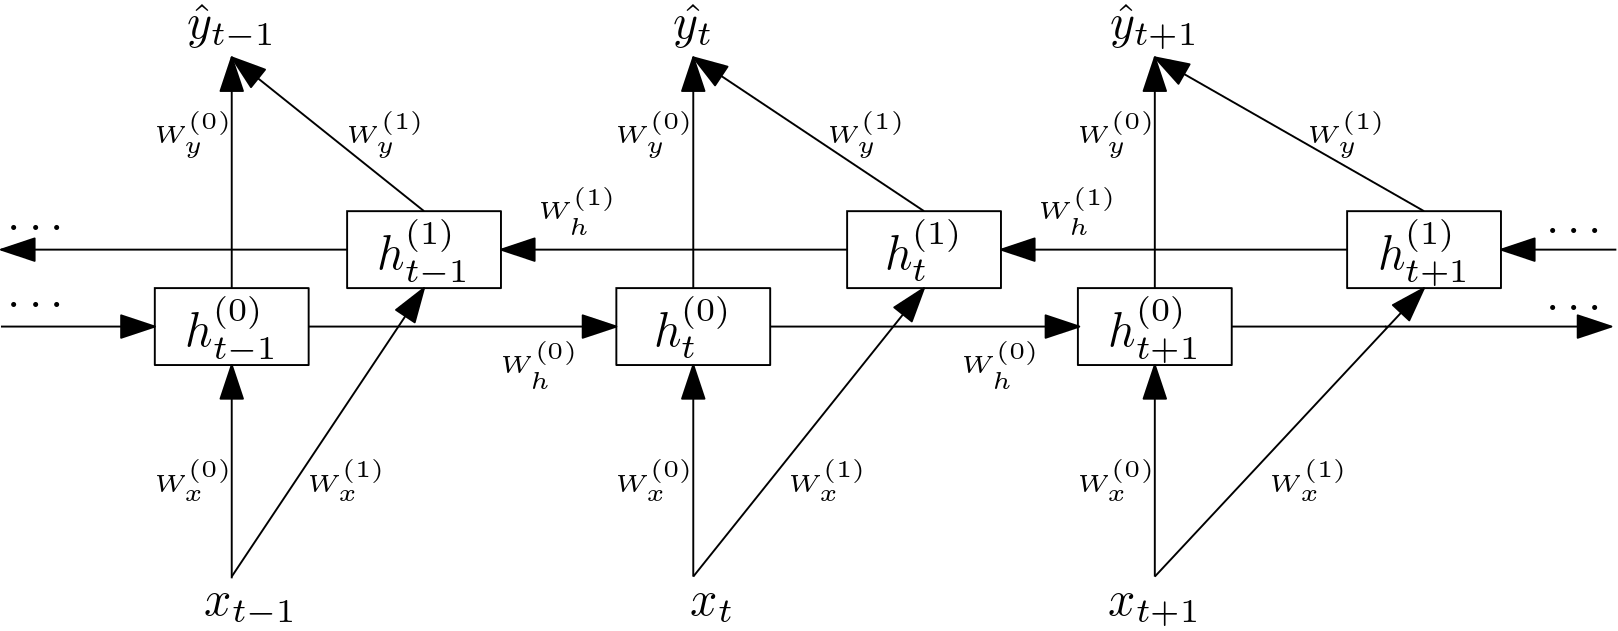
\includegraphics[width=12cm]{rnn_bi.png}
	\caption{Unrolled structure of BRNN \cite{matous}}
	\label{fig:brnn}
\end{figure}


Both hidden states are updated identically as the hidden state in RNN.

\begin{equation}
    {h_t^{(0)} = f(W_{x}^{(0)}x_t + W_{h}^{(0)}h_{t-1}+\vec{b_{h^{(0)}}})}
\end{equation}

\begin{equation}
    {h_t^{(1)} = f(W_{x}^{(1)}x_t + W_{h}^{(1)}h_{t-1}+\vec{b_{h^{(1)}}})}
\end{equation}

The output is then computed in combination of both hidden states.

\begin{equation}
    {\hat{y}_t = g(W_{y}^{(0)}h_t^{(0)} + W_{y}^{(1)}h_t^{(1)} + \vec{b_y})}
\end{equation}

All the activation functions and parameters remain the same as they were in RNN. 
